\documentclass{article}

\usepackage{graphicx}
\usepackage{tikz}
\usepackage{tikzsymbols}
\usetikzlibrary{calc,patterns,shapes.geometric}
\pagestyle{empty}
\usepackage[margin=0pt]{geometry}
\geometry{papersize={14in,12in}}

\def\centerarc[#1](#2)(#3:#4:#5){\draw[#1] ($(#2)+({#5*cos(#3)},{#5*sin(#3)})$) arc (#3:#4:#5);}

\begin{document}
	\begin{figure}
		\centering
		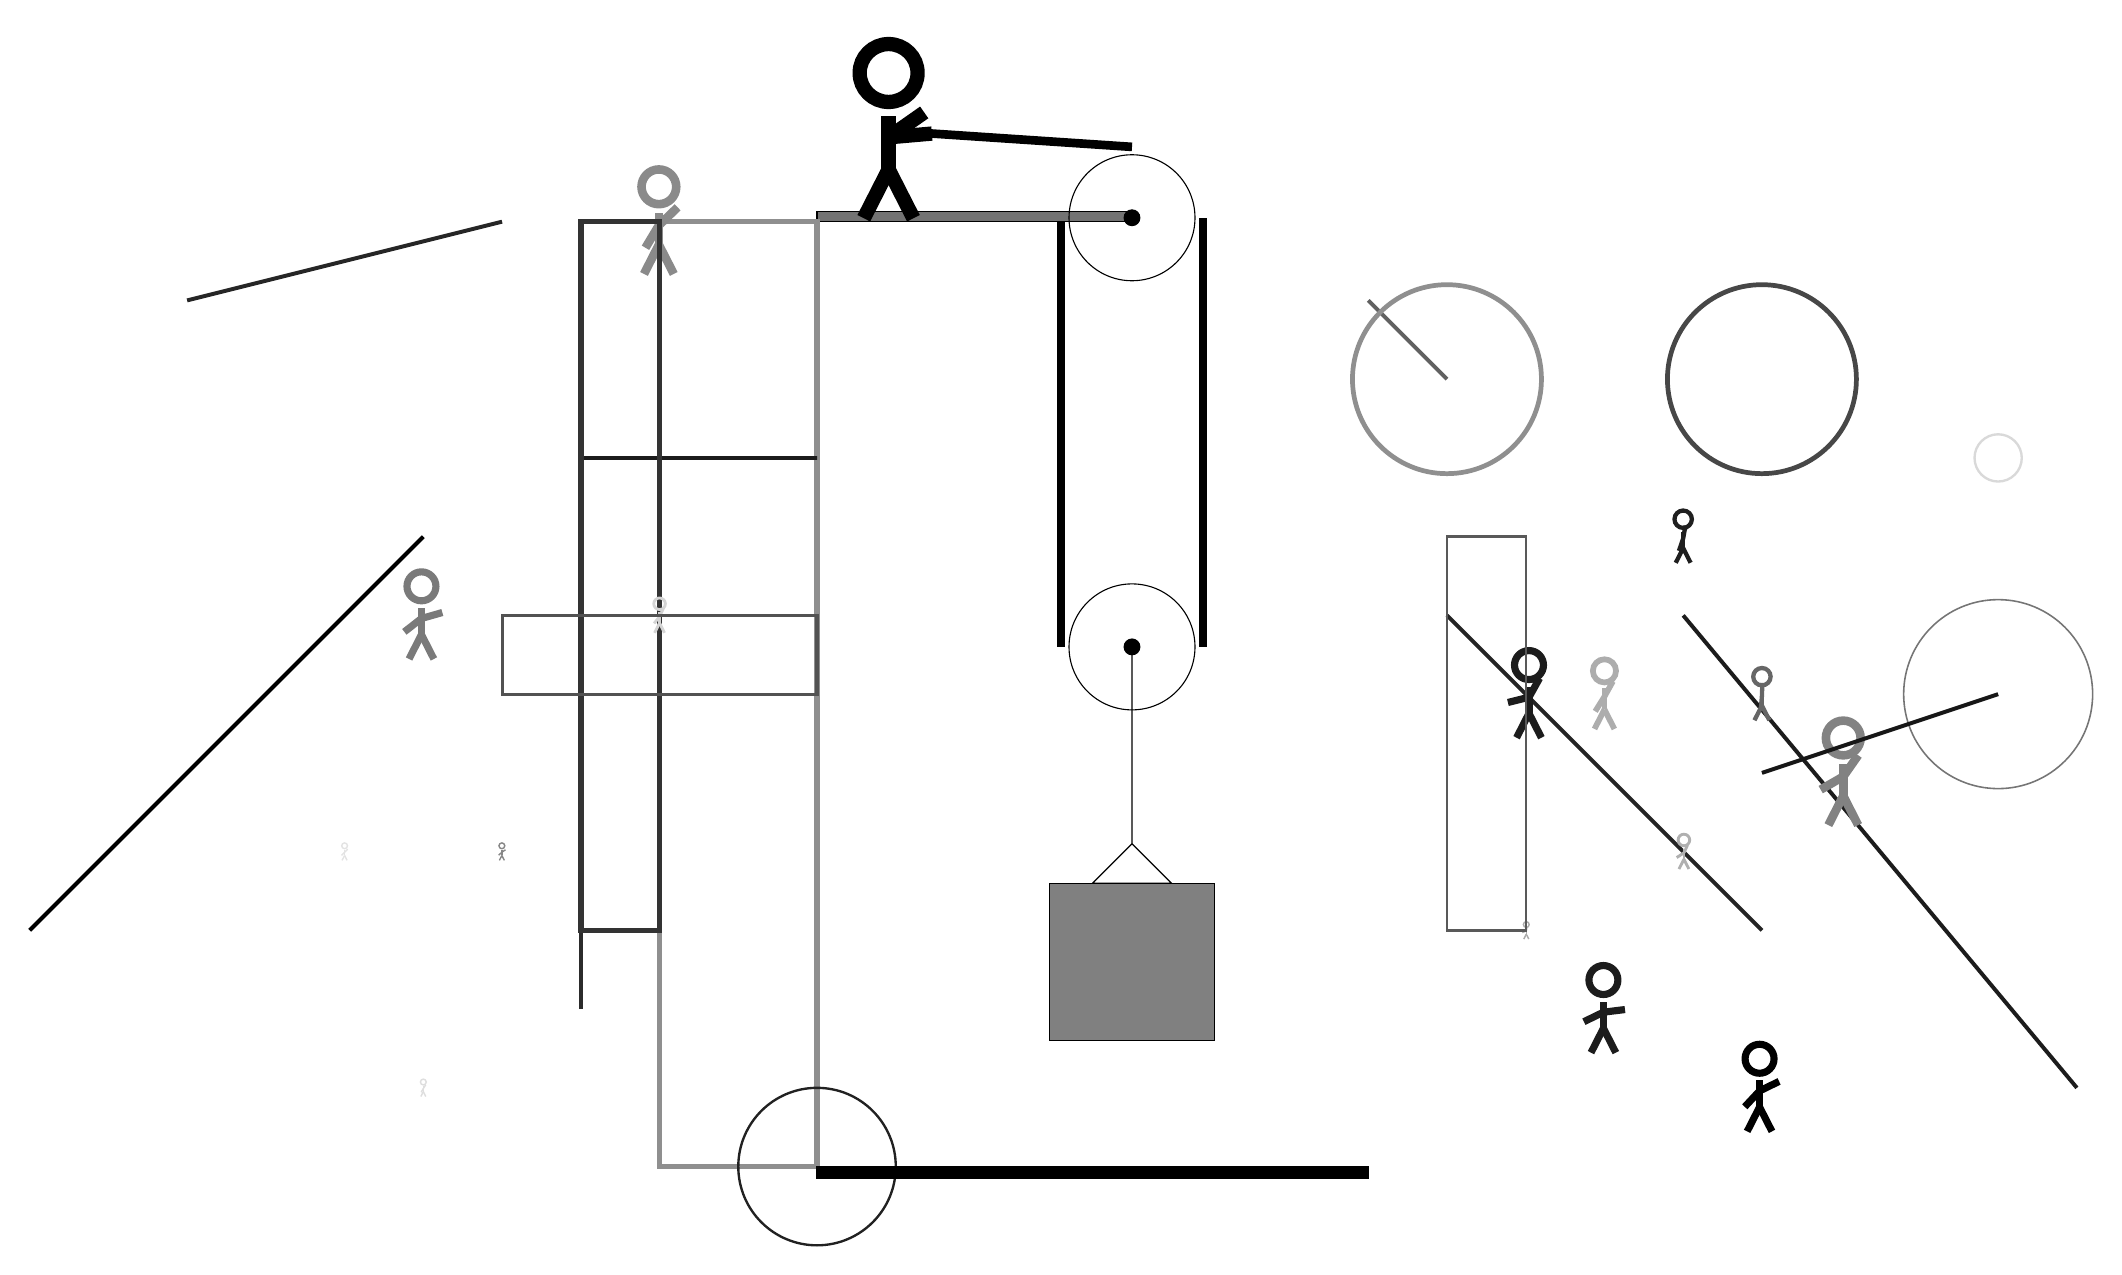
\begin{tikzpicture}
			%%%%% START %%%%%
			
			\draw[fill=black!55] (-2, 9) rectangle (2, 9.125);
			
			\draw (2, 3.6) circle (0.8);
			\draw[fill=black] (2, 3.6) circle (0.1);
			
			\draw (2, 9.05) circle (0.8);
			\draw[fill=black] (2, 9.05) circle (0.1);
			
			\draw (2, 3.6) -- (2, 1.1) -- (1.5, 0.6) -- (2.5, 0.6) -- (2, 1.1);
			\draw[fill=black!50] (0.95, 0.6) rectangle (3.05, -1.4);
			
			\draw[line width=1.1mm] (1.1, 9) -- (1.1, 3.6);
			\centerarc[line width=1.1mm](2, 3.6)(180:360:0.9);
			\draw[line width=1.1mm](2.9, 3.6) -- (2.9, 9.05);
			\centerarc[line width=1.1mm](2, 9.05)(0:90:0.9);
			\draw[line width=1.1mm](2, 9.95) -- (-1, 10.15);
			
			\node[line width=0.6mm, color=black!33] at (7, 0) {\Strichmaxerl[1][21][80]};
			
			\draw [line width=0.2mm, color=black!54](13, 3) circle (1.2);
			\draw[line width=0.5mm, color=black!86](10, 0) -- (6, 4);
			\node[line width=0.3mm, color=black!89] at (7, 3) {\Strichmaxerl[5][14][61]};
			
			\draw[line width=0.7mm, color=black!44] (-4, -3) rectangle (-2, 9);
			\draw[line width=0.5mm, color=black!89](9, 4) -- (14, -2);
			
			\draw [line width=0.6mm, color=black!72](10, 7) circle (1.2);
			
			\draw[line width=0.5mm, color=black!83](-5, -1) -- (-5, 0);
			\node[line width=0.6mm, color=black!47] at (-6, 1) {\Strichmaxerl[1][43][34]};
			\node[line width=0.7mm, color=black!60] at (10, 3) {\Strichmaxerl[3][85][88]};
			
			\draw[line width=0.5mm, color=black!85](-6, 9) -- (-10, 8);
			\node[line width=0.4mm, color=black!49] at (11, 2) {\Strichmaxerl[6][30][55]};
			\draw[line width=0.5mm, color=black!89] (-2, 6) rectangle (-5, 6);
			\node[line width=0.6mm, color=black!89] at (8, -1) {\Strichmaxerl[5][26][7]};
			\draw[line width=0.5mm, color=black!62](6, 7) -- (5, 8);
			\node[line width=0.5mm, color=black!46] at (-4, 9) {\Strichmaxerl[6][59][44]};
			\draw [line width=0.3mm, color=black!15](13, 6) circle (0.3);
			
			\node[line width=0.3mm, color=black!88] at (9, 5) {\Strichmaxerl[3][71][80]};
			\draw [line width=0.4mm, color=black!26](9, 2) circle (0.0);
			
			\draw[line width=0.5mm, color=black!100](-7, 5) -- (-12, 0);
			\draw [line width=0.6mm, color=black!44](6, 7) circle (1.2);
			
			\node[line width=0.7mm, color=black!11] at (-8, 1) {\Strichmaxerl[1][45][45]};
			\draw[line width=0.7mm, color=black!80] (-4, 9) rectangle (-5, 0);
			\node[line width=0.2mm, color=black!32] at (8, 3) {\Strichmaxerl[4][58][61]};
			\draw[line width=0.5mm, color=black!91](10, 2) -- (13, 3);
			\node[line width=0.5mm, color=black!17] at (-4, 4) {\Strichmaxerl[2][51][65]};
			
			\node[line width=0.7mm, color=black!100] at (10, -2) {\Strichmaxerl[5][47][26]};
			\node[line width=0.3mm, color=black!31] at (9, 1) {\Strichmaxerl[2][33][65]};
			
			\draw[line width=0.3mm, color=black!65] (7, 0) rectangle (6, 5);
			\draw[line width=0.4mm, color=black!68] (-2, 3) rectangle (-6, 4);
			\node[line width=0.2mm, color=black!52] at (-7, 4) {\Strichmaxerl[5][38][16]};
			
			\draw [line width=0.3mm, color=black!87](-2, -3) circle (1.0);
			\node[line width=0.3mm, color=black!13] at (-7, -2) {\Strichmaxerl[1][60][57]};
			
			\node at (-1, 10.15) {\Strichmaxerl[10][-175][35]};
			
			\draw[fill=black] (-2, -3) rectangle (5, -3.15);
			
			%%%%% END %%%%%
		\end{tikzpicture}
	\end{figure}	
\end{document}